\chapter{Etude du réseau complet}
Dans ce chapitre, nous allons étendre l'étude précédente à l'ensemble du réseau.
Nous allons commencer par une étude générale du réseau puis, nous étudierons les pire temps de traversé (WCTT) et les pires différences des volumes de données du réseau (backlog). Pour fini, nous verrons comment améliorer le WCTT et le backlog du réseaux.
\section{Analyse générale du réseau}
Dans un premier temps, nous allons calculer les courbes d'arrivées de B et C, puis les courbes de service des ports de sorties de B et C.
\subsection{Courbes d’arrivées de B et C}
Nous avons calculé les courbes d'arrivées des flux $v_3$, $v_4$ et $v_5$, c'est-à-dire le volume de données qui arrive par intervalle de temps dans les entrées du bloc C et par la troisième entrée du bloc B. Respectivement : 
\begin{description}
\item[$\alpha_3^{C1}$ ] Qui est la même que $\alpha_1^{A1}$, dans le chapitre précédent, figure \ref{fig:CA_1_2}, page \pageref{fig:CA_1_2}. En effet $v_1$ et $v_3$ ont les mêmes caractéristiques (BAG et $s_{max}$). Elle est de type sceau percé.

\item[$\alpha_4^{C1}$ ] Qui est la même que $\alpha_2^{A1}$, dans le chapitre précédent, figure \ref{fig:CA_1_2}, page \pageref{fig:CA_1_2}. En effet $v_2$ et $v_4$ ont les mêmes caractéristiques (BAG et $s_{max}$). Elle est de type sceau percé.

\item[$\alpha_5^{B1}$ ] Qui doit réponde aux  caractéristiques suivantes : BAG$=128 ms$ et $s_{max}=800$ octets. Elle est représentée figure \ref{fig:CA_5}. Elle est de type sceau percé.
\end{description}

\begin{figure}[!ht]
\centering
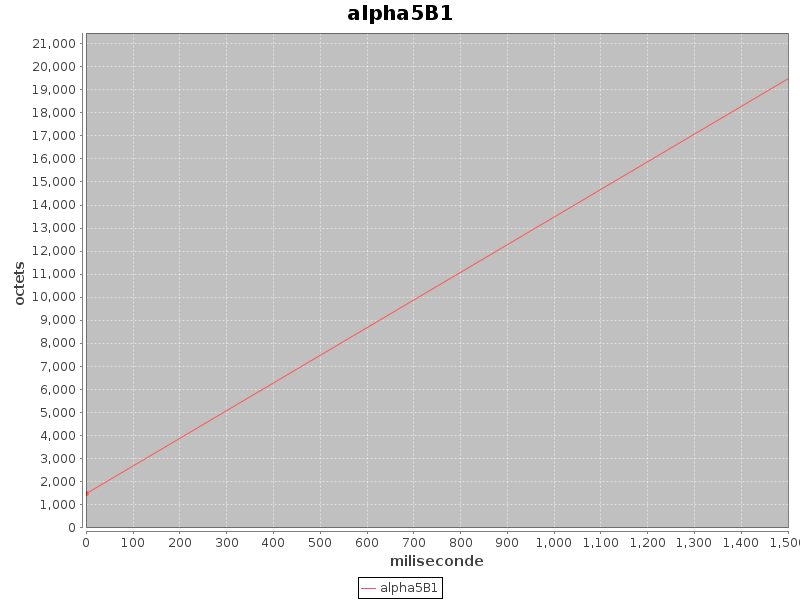
\includegraphics[width = .6\textwidth]{./II/images/alpha_5.png}
\caption{\label{fig:CA_5}Courbe d'arrivée $\alpha$ du flux $v_5$ (bleu)}
\end{figure} 
\subsection{Courbes de service de B et C}
Nous allons voir ici, par la même méthode que celle utilisé dans le chapitre précédent, les courbes de services des deux sorties de B et la sortie de C. Voici, en commençant par la courbe de service du n\oe ud C :
\begin{description}
\item[$\beta^{C1}$] Qui est la même que $\beta^A$, dans le chapitre précédent, figure \ref{fig:serviceA}, page \pageref{fig:serviceA}. En effet les n\oe uds A et C ont les mêmes caractéristiques, la courbe de service est donc identique.
\item[$\beta^{B1}$ et $\beta^{B2}$] Les courbes de services de B sont identiques à celle de C car les n\oe uds ont tous les mêmes propriétés. 
\end{description}

\subsection{Étude de l'ensemble du réseau}
%1)) Calculer alpha^A1, la courbe d’arrivée du port de sortie 1 de A à partir des courbes d’arrivée par flux alpha_1^A1 1 et alpha_2^A1.
% alpha'^A déja fait avant en flux séparés 
% alpha'^C avec alpha^C = alpha_1^C + alpha_2^C et beta_C
% alpha'^B1 avec alpha^C = alpha_1^C + alpha_2^C et beta_C
Pour réaliser les courbes d'arrivées de tous les flux de sortie du réseau, nous avons décidé de calculer $\alpha'^C$ en considérant $\alpha^C = \alpha_1^C + \alpha_2^C$. Pour le calcul de $\alpha'^{B1}$ et $\alpha'^{B2}$, nous avons décidé de faire un calcul avec les flux séparés.
Voici la courbe d'arrivée de $\alpha'^C = \alpha^C \varoslash \beta_C$ : 
\begin{figure}[!ht]%
\begin{minipage}{.48\textwidth}%
\centering%
\noindent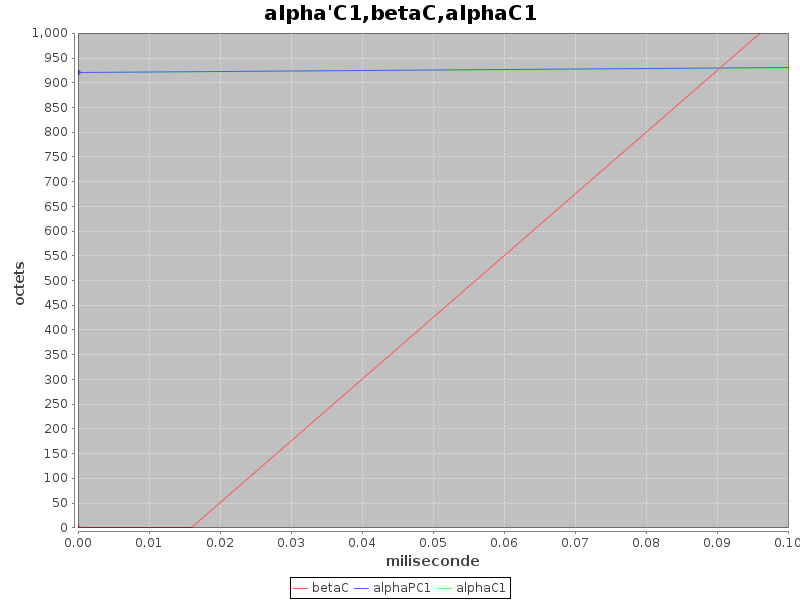
\includegraphics[width = \textwidth]{./II/images/alphaP_C1.png}%
\caption{\label{fig:CS_C}Courbe de sortie $\alpha'_C$ (bleu), $\alpha_C$ (vert) et la courbe de service $\beta_C$ (rouge) de C.}%
\end{minipage}\hfill%
\begin{minipage}{.48\textwidth}%
\centering%
\noindent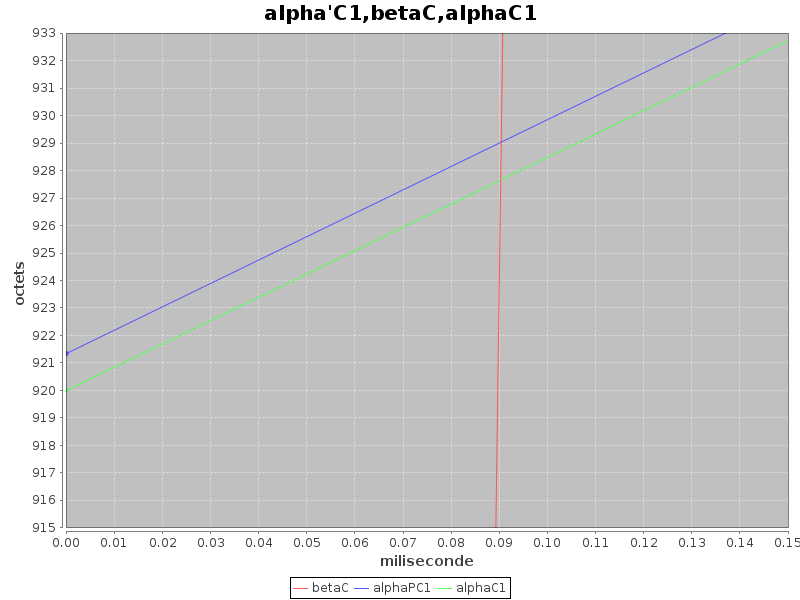
\includegraphics[width = \textwidth]{./II/images/alphaP_C1-2.png}%
\caption{\label{fig:CS_C-2}Zoom de la figure \ref{fig:CS_C}.}%
\end{minipage}%
\end{figure} 


Courbe de sortie de la première sortie de B: 
\begin{figure}[!ht]%
% alpha1PB1 et alpha3PB1
\begin{minipage}{.48\textwidth}%
\centering%
\noindent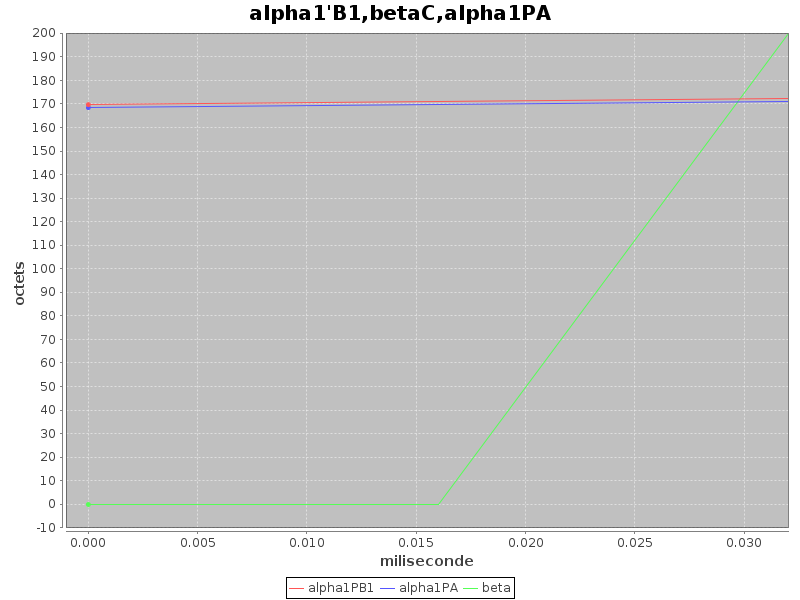
\includegraphics[width = \textwidth]{./II/images/alpha1PB1.png}%
\caption{\label{fig:alpha1PB1}Courbe de sortie $\alpha_{1}^{'B1}$ (bleu), $\alpha_{1} ^{'A}$ (vert) et la courbe de service $\beta_B$ (rouge) de B.}%
\end{minipage}\hfill%
\begin{minipage}{.48\textwidth}%
\centering%
\noindent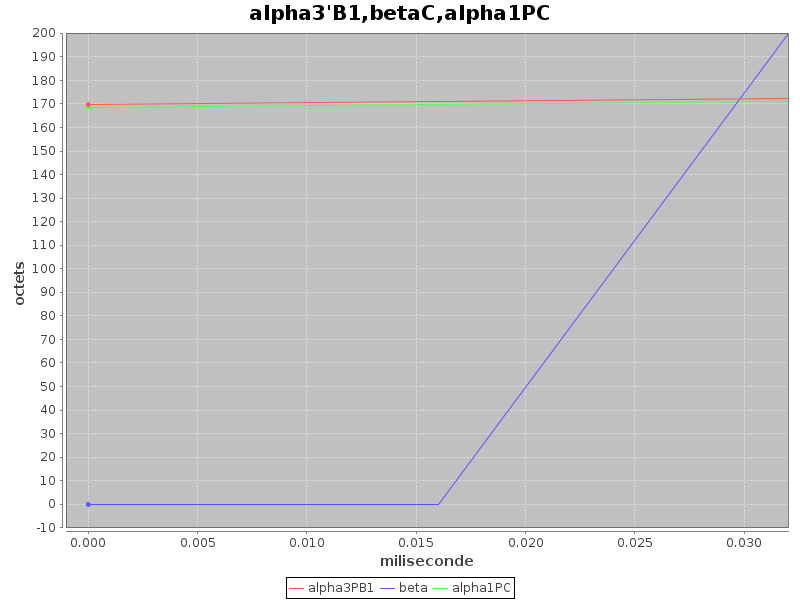
\includegraphics[width = \textwidth]{./II/images/alpha3PB1.png}%
\caption{\label{fig:alpha3PB1}Courbe de sortie $\alpha_3 ^{'B1}$ (bleu), $\alpha_1^{'C}$ (vert) et la courbe de service $\beta_B$ (rouge) de B.}%
\end{minipage}\vspace{5mm}\newline 
%
% alpha4PB1 et alpha5PB1
\begin{minipage}{.48\textwidth}%
\centering%
\noindent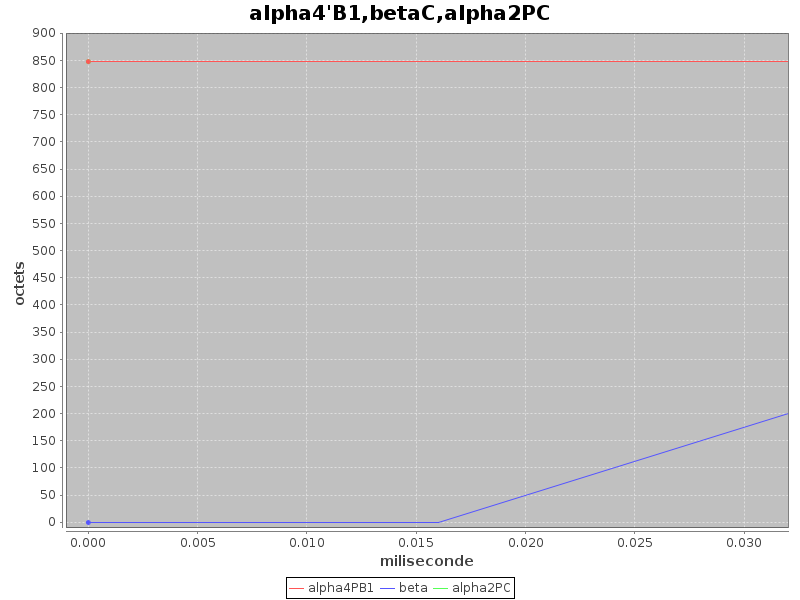
\includegraphics[width = \textwidth]{./II/images/alpha4PB1.png}%
\caption{\label{fig:alpha4PB1}Courbe de sortie $\alpha_4^{'B1}$ (bleu), $\alpha_2^{'C}$ (vert) et la courbe de service $\beta_B$ (rouge) de C.}%
\end{minipage}\hfill%
\begin{minipage}{.48\textwidth}%
\centering%
\noindent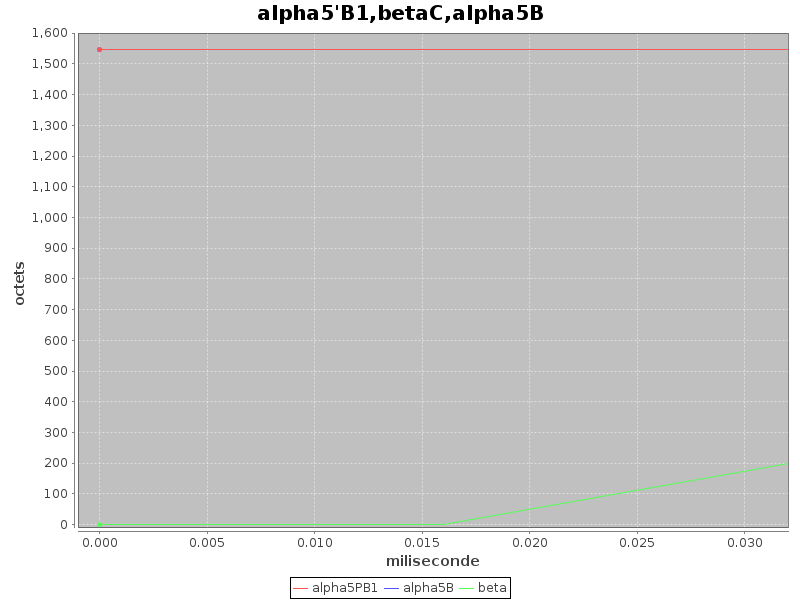
\includegraphics[width = \textwidth]{./II/images/alpha5PB1.png}%
\caption{\label{fig:alpha5PB1}Courbe de sortie $\alpha_5^{'B1}$ (bleu), $\alpha_5^{B}$ (vert) et la courbe de service $\beta_B$ (rouge) de C.}%
\end{minipage}%
\end{figure} 

Courbe de sortie de la seconde sortie de B: 
\begin{figure}[!ht]%
%  alpha2PB2
\centering%
\noindent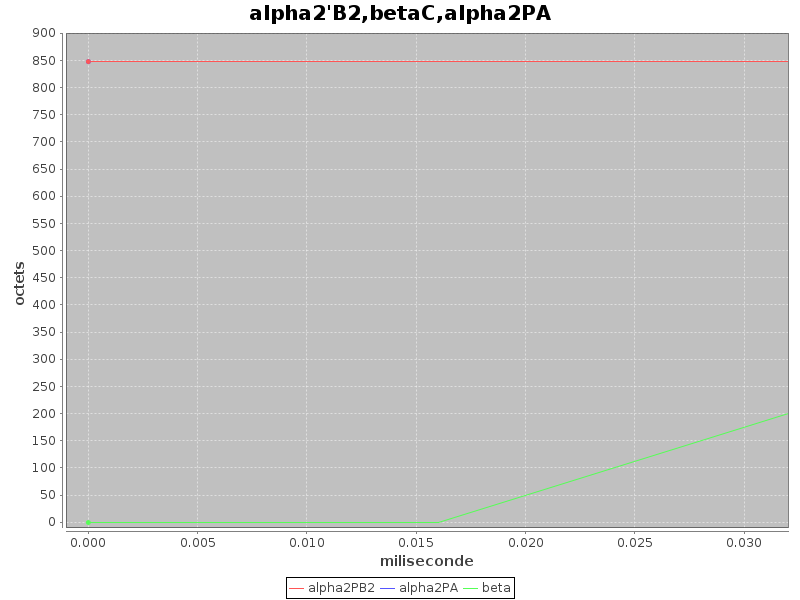
\includegraphics[width = .4\textwidth]{./II/images/alpha2PB2.png}%
\caption{\label{fig:alpha2PB2}Courbe de sortie $\alpha_2^{'B2}$ (bleu), $\alpha_2^{'A}$ (vert) et la courbe de service $\beta_B$ (rouge) de C.}%
\end{figure} 
%2)) Calculer le délai pire-cas tau_A1 et le backlog pire-cas mu_A1 du port de sortie de A à partir de alpha^A1 et de beta^A.
Nous avons ensuite calculer les délais pire-cas 
%3)) Calculer alpha_1^B1 et alpha_2^B2 les courbes d’arrivée des ports de sortie 1 et 2 de B par flux.

%4)) Calculer alpha^B1 et alpha^B2 les courbes d’arrivée des ports de sortie de B en prenant en compte les flux de manière séparée.

%5)) Calculer alpha^B1 et alpha^B2 les courbes d’arrivée des ports de sortie de B en prenant en compte la sérialisation des flux.


\section{Borne sur les pires temps de traversée et sur le pire backlog}

\subsection{Pire délai de traversée de bout-en bout}

\subsection{Pire backlog du réseau}

\section{Amélioration du pire délai de traversée de bout-en bout}
\subsection{Dépendance des flux et tracé des nouvelles courbes}
\subsection{Re-calcul des délais pire cas et conclusion}